\subsection{Contexto geográfico de los sistemas y áreas}

El cuaderno \texttt{micode.ipynb} incluye dos mapas que permiten situar geográficamente la información eléctrica del conjunto de datos. El primero representa la red troncal de transmisión del Sistema Eléctrico Nacional (SEN) en 2023; el segundo muestra los enlaces entre regiones al 31 de diciembre del mismo año. Ambos se reproducen como contexto territorial y corresponden a una fecha distinta del periodo de 2022 seleccionado para OLS.

\begin{figure}[p]
\centering
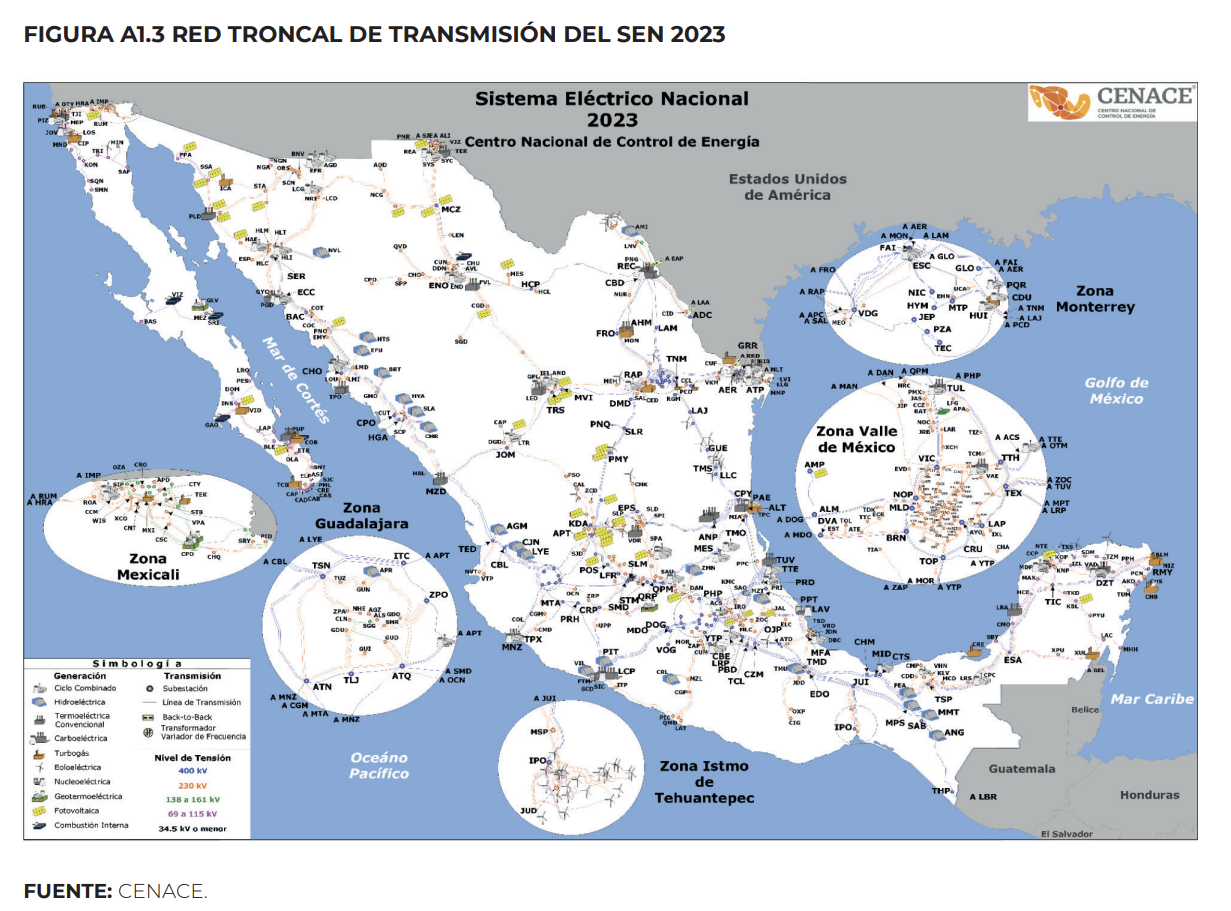
\includegraphics[width=\textwidth,height=0.72\textheight,keepaspectratio]{figuras/04_metodologia/red_troncal_sen_2023.png}
\caption{Red troncal de transmisión del SEN en 2023. Imagen incorporada en \texttt{micode.ipynb}, figura AI.3. La fuente indicada en la imagen es CENACE.}
\label{fig:red-troncal-sen}
\end{figure}

La figura~\ref{fig:red-troncal-sen} presenta la distribución de infraestructura de generación y transmisión, con símbolos para diferentes tecnologías y niveles de tensión. Sus ampliaciones permiten observar zonas como Mexicali, Guadalajara, Monterrey, Valle de México e Istmo de Tehuantepec. Este contexto ayuda a interpretar las columnas de sistema y área como identificadores territoriales del registro eléctrico.

\begin{figure}[p]
\centering
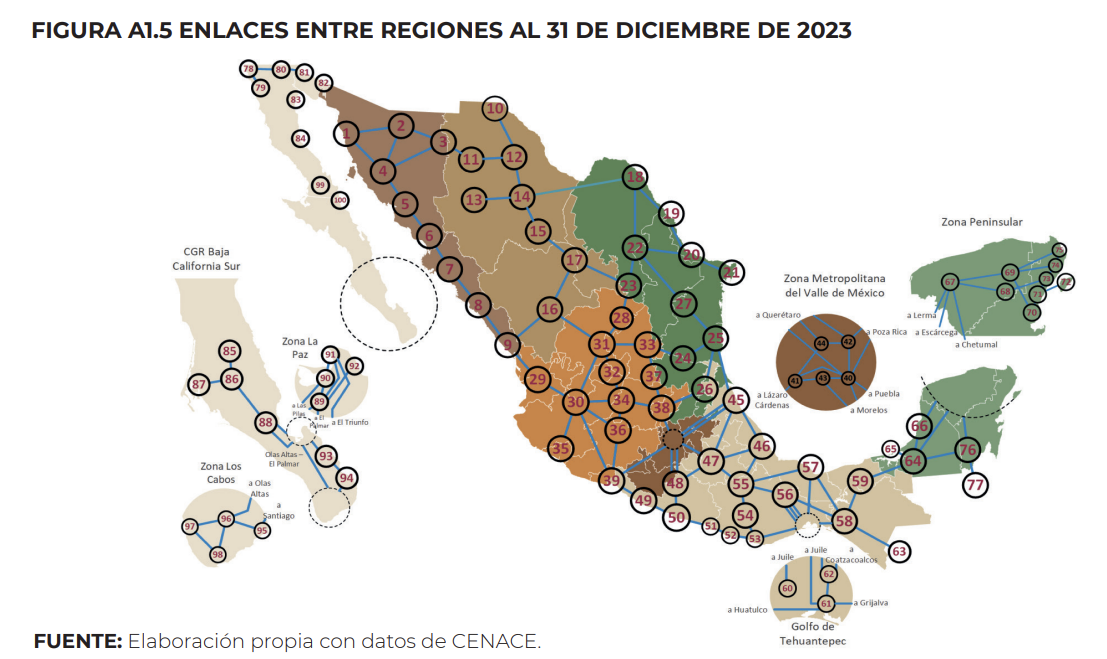
\includegraphics[width=\textwidth,height=0.68\textheight,keepaspectratio]{figuras/04_metodologia/enlaces_regiones_2023.png}
\caption{Enlaces entre regiones al 31 de diciembre de 2023. Imagen incorporada en \texttt{micode.ipynb}, figura AI.5. El crédito original señala una elaboración con datos de CENACE; el mapa se reproduce del cuaderno y no constituye una elaboración de esta tesis.}
\label{fig:enlaces-regiones}
\end{figure}

La figura~\ref{fig:enlaces-regiones} representa regiones numeradas y los enlaces dibujados entre ellas, e incluye detalles de Baja California Sur y de la Zona Metropolitana del Valle de México. Los números del mapa no deben interpretarse como equivalentes directos a los nueve códigos de área del archivo, pues esa correspondencia requiere información adicional.

En las salidas del cuaderno se identifican los sistemas BCA, BCS y SIN, así como las áreas BCA, BCS, CEN, NES, NOR, NTE, OCC, ORI y PEN. Los mapas complementan la descripción de estos registros. El modelo OLS utiliza la generación de una sola área y no incorpora coordenadas, distancias ni enlaces de transmisión como variables predictoras.
